\section{Software Defined WAN}

\subsection{Introduction}
Traditional WAN solutions have challenges to solve. 
Often MPLS circuits are used. New policies have to be applied on each device. 
Adding new sites is expensive.  
Configuration is distributed and deployed as a template.
Failover is dependent on the state of a link, outages introduce latency (convergence of traditional routing protocols). 

All of this hinders growth and agility.

SD-WAN aims to reduce these problems by eliminating the need for MPLS circuits, offloading user traffic to the cloud, 
simplify deployment and management, as well as centralize visiblity and controls. 

\begin{figure}[h]
    \centering
    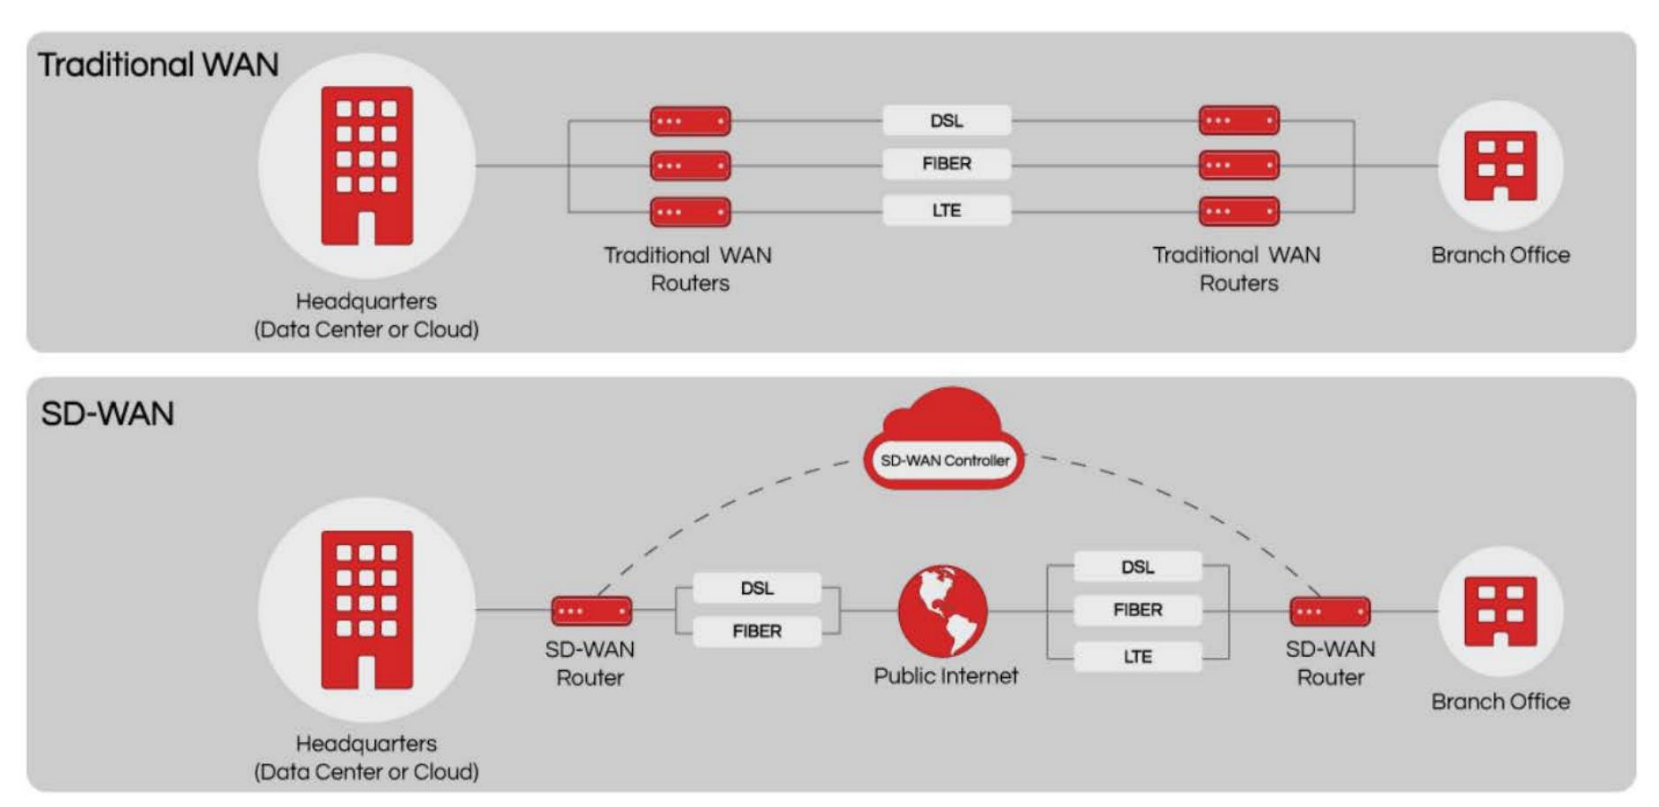
\includegraphics[width=\textwidth]{sdwan-vs-traditionalwan.png}
    \caption{Traditional WAN vs. SD-WAN}
\end{figure}

\subsubsection{SD-WAN vs SASE}

SASE Secure Access Service Edge. Focus us on Cloud Services, datacenter is ``just another branch office''. Conbines the capabilities of a WAN with comprehensive security functions 
(secure web gateway, firewall as a service, etc.) to facilitate secure network access in cloud and mobile environments. 
Best practices include a zero trust approach. 

SDWAN is a software-based approach to building and maintaining networks that connect geographically dispersed offices. 
Focus is on the datacenter.
\subsubsection{Bottleneck Security}
Traffic crossing the cloud is a risk. Every branch has direct internet access, split tunneling must be applied correctly. 
IoT / BYOD devices connected to the cloud. 

While these challenges exist, traditional security is not built for the cloud. 
It usually lacks in terms of performance, flexibility and scalability.

The traditional security model usually steers all traffic via some central device applying security features.
This creates a bottleneck for traffic, that would otherwise not have to cross this central point. 

\begin{figure}[h]
    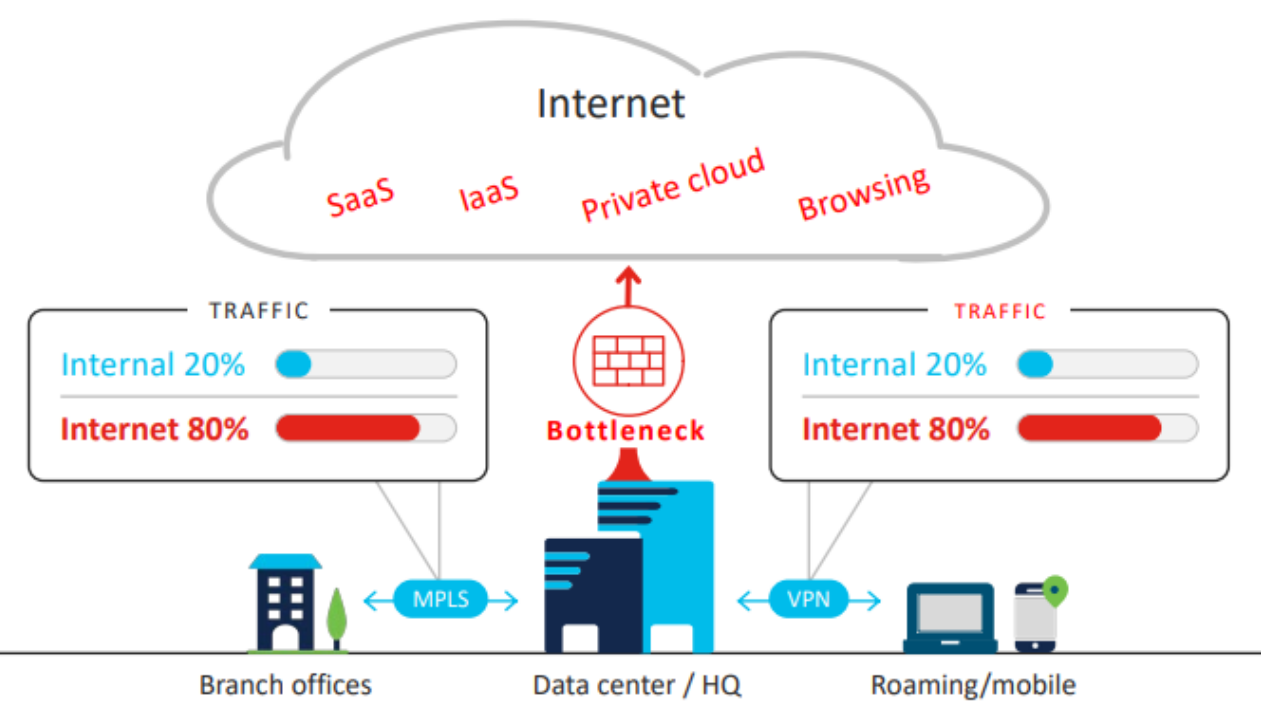
\includegraphics[width=\textwidth]{sdwan-bottleneck-security.png}
    \caption{Central security features as bottleneck}
\end{figure}

\subsubsection{SD-WAN Advantages}
Cisco SD-WAN approach centralizes the management of reachability, security and application policies.
It uses a single extensible control plane to manage all WAN-edge devices. Instead of having to create a full mesh 
connection topology between all WAN-edge devices, each device only has to be set up to connect to the controller.
Everything else is automated. This dramatically lowers complexity and increases overall solution scale.

\subsection{Cisco SD-WAN Components}

\subsubsection{vSmart}
Facilitates fabric discovery. Distributes data plane and app-aware routing policies to the vEdge routers. 
Involved only in control plane communication, reducing the complexity. 
Eliminates the need for full-mesh routing on the transport side.

Highly resilient -- usually several instances are deployed.  

\subsubsection{vEdge}
WAN-Edge router, provides secure data plane with all other vEdge routers.
Implements application-aware routing policies, using standards-based routing protocols (OSPF and BGP)
 and VRRP for first-hop redundancy.
Establishes secure control plane with vSmart controllers using OMP.
Exports performance statistics.

Supports zero-touch deployment and comes in physical or virtual form factor.

\subsubsection{vManage}
Graphical user interface, single point of management for daily operations. 
Provides a GUI with Role-Based Access as well as REST and NETCONF Interfaces.
Centralized provisioning, troubleshooting and monitoring.

Highly resilient.

\subsubsection{vBond}
Only used on first connect of a newly registered device. MAC Address of vEdge device must be associated with a cisco account 
to ensure correct assignment.

Orchestrates control and management plane, first point of authentication. Distributes a list of vSmart and vManage controllers to 
all vEdge routers.  

Requires a publicly reachable IP address.

\subsubsection{OMP - Overlay Management Protocol}
Unified control plane, TCP-based extensible control plane protocol.
Runs between vEdge routers and vSmart controllers, as well as between vSmart controllers themselves.
Advertises control plane context.

\subsection{Dataplane Operations}

Data Plane security is enforced by the creation of IPSec tunnels between all vEdge routers.
Encryptino is symmetric with the SD-WAN Control plane facilitating the encryption key exchange.

IP Sec by default uses Authentication Header AH and Encapsulating Security Protocol ESP. 

\subsubsection{BFD - Bidirectional Forwarding Detection}
Path liveliness and quality measurement detection protocol. Used to determine the quality of WAN paths and 
make forwarding decisions according to traffic SLA policies.

Supported Metrics are Up/Down, Loss, Latency, Jitter and IPSec tunnel maximum MTU.

Runs between vEdge and vEdge Cloud routers, inside IPSec tunnels. It is invoked automatically at 
tunnel establishment and cannot be disabled.

Uses hello interval, poll interval and multiplier for detection.

\subsubsection{Application Visibility and Recognition}
Deep Packet Inspection enables the use of detailed SLA for each application, which can be enforced using the path 
liveliness measures performed by the BFD protocol. 

\subsection{Cloud developments}
\begin{itemize}
    \item \textbf{Direct Internet Access:} Can use one or more local ``DIA'' exits or route traffic to the regional 
    hub through the SD-WAN fabric and exit to the internet from there. Can be a VPN default route to ensure DIA for all traffic, or use a data policy for selective traffic DIA.
    NAT on the vEdge router allows only response traffic for established connections. All other traffic from the internet will be blocked.
    \item \textbf{Cloud Attached Compute, Cloud Gateway VPC/VNET:} \\
    vEdge cloud routers can be instantiated in Amazon VPCs or MS Azure VNETs. 
\end{itemize}

\subsection{SDW-WAN Overlay Routing}
OMP learns and translates routing information across the VPN overlay.

Route types include 
\begin{itemize}
    \item OMP routes: Prefixes learned from site-local, similar to BGP Prefixes. Can be directly connected, static, BGP or OSPF learned routes.
        They advertise several attributes like TLOC, Site ID, VPN ID, Tag, Preference, Originator ID and Origin.
    \item TLOCs: Transport Locators. Ties OMP route to physical location (vEdge), similar to BGP next-hop. 
        3-Tuple identifier: (system-ip, color, encapsulation type).
    \item Service routes: ties OMP routes to an advertised network service like firewall, load balancer or IDP.
\end{itemize}